
\documentclass[12pt,a4paper]{article}

% Margins.
\setlength{\oddsidemargin}{0in}
\setlength{\evensidemargin}{0in}
\setlength{\headheight}{12pt}
\setlength{\headsep}{0pt}
\setlength{\topmargin}{-60pt}
\setlength{\textwidth}{6.5in}
\setlength{\textheight}{10.75in}

\usepackage{amsmath}
\usepackage{float}
\usepackage{graphicx}
\usepackage[hyphens]{url}
\usepackage{hyperref}	% Clickable links to figures, references and urls.
\usepackage{datetime}
\usepackage{longtable}
\usepackage{subfigure}

% Drawing.
\usepackage{pgf}
\usepackage{tikz}

% Listings for formatting code.
\usepackage{listings}
\usepackage{textcomp}
% General options.
\lstset{breaklines=true, basicstyle=\small\ttfamily, tabsize=4, numbers=left, stepnumber=1, frame=single, showstringspaces=false, upquote=true}
% C++ specific high-lighting. Comments are 50/50 shades of green/black and strings coloured with 60/40 red/black mixture.
\lstset{language=[ISO]C++, commentstyle=\color{green!50!black}, keywordstyle=\color{blue}, stringstyle=\color{red!60!black}}

%opening
\title{Data Structures and Algorithms\\Class 36\\Parallelism}
\author{Attique Dawood}
\date{May 12, 2015\\[0.2cm] Last Modified: \today, \currenttime}
\begin{document}
\maketitle
\section{Announcements}
\begin{itemize}
\item None.
\end{itemize}
\section{Revision}
\begin{itemize}
\item Network programming.
\end{itemize}
\section{Task--Parallelism\index{parallelism!task}}
In task--parallelism computation consist of several independent tasks that run concurrently. These tasks may be completely unrelated but the end result is dependent on their outputs. Consider summation of a series, where we want to compute the value of $e^x$ from Taylor series. The mathematical expression is given by
\begin{equation}
e^x = 1+\dfrac{x^1}{1!}+\dfrac{x^2}{2!}+\dfrac{x^3}{3!}+\dfrac{x^4}{4!}+\dfrac{x^5}{5!}+\dfrac{x^6}{6!}+...+\dfrac{x^n}{n!}
\label{eq:ex-Taylor-Series}
\end{equation}
\begin{figure}[h]
\centering
\subfigure[Single--threaded implementation]{
\begin{tikzpicture}
	\newcommand{\Xdisp}{0cm}
	\newcommand{\Ydisp}{0cm}
	% e^x;
	\coordinate [label=center:$e^x\rightarrow$] (exequals) at (\Xdisp-0.75cm,\Ydisp+0.75cm);
	% Single-threaded flow chart.
	\draw (\Xdisp-0.25cm,\Ydisp+0.75cm) -- (\Xdisp+0.5cm,\Ydisp+0.75cm) -- (\Xdisp+0.5cm,\Ydisp);
	\draw (\Xdisp,\Ydisp) rectangle (\Xdisp+1.0cm,\Ydisp-1.0cm);
	\coordinate [label=center:$\dfrac{x^0}{0!}$] (Term0ST) at (\Xdisp+0.5cm,\Ydisp-0.5cm);

	\renewcommand{\Xdisp}{1.25cm}
	\renewcommand{\Ydisp}{-1.25cm}
	\draw (\Xdisp-0.25cm,\Ydisp+0.75cm) -- (\Xdisp+0.5cm,\Ydisp+0.75cm) -- (\Xdisp+0.5cm,\Ydisp);
	\draw (\Xdisp,\Ydisp) rectangle (\Xdisp+1.0cm,\Ydisp-1.0cm);
	\coordinate [label=center:$\dfrac{x^1}{1!}$] (Term1ST) at (\Xdisp+0.5cm,\Ydisp-0.5cm);
	\filldraw[fill=white] (\Xdisp+0.5cm,\Ydisp+0.75cm) circle (0.25cm);
	\coordinate [label=center:$+$] (plusTerm1ST) at (\Xdisp+0.5cm,\Ydisp+0.75cm);

	\renewcommand{\Xdisp}{2.5cm}
	\renewcommand{\Ydisp}{-2.5cm}
	\draw (\Xdisp-0.25cm,\Ydisp+0.75cm) -- (\Xdisp+0.5cm,\Ydisp+0.75cm) -- (\Xdisp+0.5cm,\Ydisp);
	\draw (\Xdisp,\Ydisp) rectangle (\Xdisp+1.0cm,\Ydisp-1.0cm);
	\coordinate [label=center:$\dfrac{x^2}{2!}$] (Term2ST) at (\Xdisp+0.5cm,\Ydisp-0.5cm);
	\filldraw[fill=white] (\Xdisp+0.5cm,\Ydisp+0.75cm) circle (0.25cm);
	\coordinate [label=center:$+$] (plusTerm2ST) at (\Xdisp+0.5cm,\Ydisp+0.75cm);

	\renewcommand{\Xdisp}{3.75cm}
	\renewcommand{\Ydisp}{-3.75cm}
	\draw (\Xdisp-0.25cm,\Ydisp+0.75cm) -- (\Xdisp+0.5cm,\Ydisp+0.75cm) -- (\Xdisp+0.5cm,\Ydisp);
	\draw (\Xdisp,\Ydisp) rectangle (\Xdisp+1.0cm,\Ydisp-1.0cm);
	\coordinate [label=center:$\dfrac{x^3}{3!}$] (Term3ST) at (\Xdisp+0.5cm,\Ydisp-0.5cm);
	\filldraw[fill=white] (\Xdisp+0.5cm,\Ydisp+0.75cm) circle (0.25cm);
	\coordinate [label=center:$+$] (plusTerm3ST) at (\Xdisp+0.5cm,\Ydisp+0.75cm);

	\renewcommand{\Xdisp}{5cm}
	\renewcommand{\Ydisp}{-5cm}
	\draw[dashed] (\Xdisp-0.25cm,\Ydisp+0.75cm) -- (\Xdisp+0.5cm,\Ydisp+0.75cm) -- (\Xdisp+0.5cm,\Ydisp);
	\draw (\Xdisp,\Ydisp) rectangle (\Xdisp+1.0cm,\Ydisp-1.0cm);
	\coordinate [label=center:$\dfrac{x^n}{n!}$] (TermnST) at (\Xdisp+0.5cm,\Ydisp-0.5cm);
	\filldraw[fill=white] (\Xdisp+0.5cm,\Ydisp+0.75cm) circle (0.25cm);
	\coordinate [label=center:$+$] (plusTermnST) at (\Xdisp+0.5cm,\Ydisp+0.75cm);
	% Result
	\coordinate [label=right:$\rightarrow$\textsf{Result}] (ResultST) at (\Xdisp+1.0cm,\Ydisp-0.5cm);
	% Thread.
	\draw[thick, rounded corners, ->, >=stealth] (-0.75cm,-0.5cm) -- (-0.9cm,-0.75cm) -- (-0.6cm,-1.25cm) -- (-0.9cm,-1.75cm) -- (-0.6cm,-2.25cm) -- (-0.9cm,-2.75cm) -- (-0.6cm,-3.25cm) -- (-0.9cm,-3.75cm) -- (-0.6cm,-4.25cm) -- (-0.9cm,-4.75cm) -- (-0.75cm,-5.0cm) -- (-0.75cm,-5.5cm);
\end{tikzpicture}}
\subfigure[Multi--threaded implementation]{
\begin{tikzpicture}
	\newcommand{\Xdisp}{0cm}
	\newcommand{\Ydisp}{0cm}
	% e^x;
	\coordinate [label=center:$e^x\rightarrow$] (exequals) at (\Xdisp-0.75cm,\Ydisp+0.75cm);
	% Single-threaded flow chart.
	\draw (-0.25cm,\Ydisp+0.75cm) -- (\Xdisp+0.5cm,\Ydisp+0.75cm) -- (\Xdisp+0.5cm,\Ydisp);
	\draw (\Xdisp,\Ydisp) rectangle (\Xdisp+1.0cm,\Ydisp-1.0cm);
	\coordinate [label=center:$\dfrac{x^0}{0!}$] (Term0MT) at (\Xdisp+0.5cm,\Ydisp-0.5cm);

	\renewcommand{\Xdisp}{2cm}
	\draw (-0.25cm,\Ydisp+0.75cm) -- (\Xdisp+0.5cm,\Ydisp+0.75cm) -- (\Xdisp+0.5cm,\Ydisp);
	\draw (\Xdisp,\Ydisp) rectangle (\Xdisp+1.0cm,\Ydisp-1.0cm);
	\coordinate [label=center:$\dfrac{x^1}{1!}$] (Term1MT) at (\Xdisp+0.5cm,\Ydisp-0.5cm);

	\renewcommand{\Xdisp}{4cm}
	\draw (-0.25cm,\Ydisp+0.75cm) -- (\Xdisp+0.5cm,\Ydisp+0.75cm) -- (\Xdisp+0.5cm,\Ydisp);
	\draw (\Xdisp,\Ydisp) rectangle (\Xdisp+1.0cm,\Ydisp-1.0cm);
	\coordinate [label=center:$\dfrac{x^2}{2!}$] (Term2MT) at (\Xdisp+0.5cm,\Ydisp-0.5cm);

	\renewcommand{\Xdisp}{6cm}
	\draw (-0.25cm,\Ydisp+0.75cm) -- (\Xdisp+0.5cm,\Ydisp+0.75cm) -- (\Xdisp+0.5cm,\Ydisp);
	\draw (\Xdisp,\Ydisp) rectangle (\Xdisp+1.0cm,\Ydisp-1.0cm);
	\coordinate [label=center:$\dfrac{x^3}{3!}$] (Term3MT) at (\Xdisp+0.5cm,\Ydisp-0.5cm);

	% Dots.
	\coordinate [label=center:\textsf{{\Large ...}}] (Dots1) at (8cm,\Ydisp-0.5cm);
	\coordinate [label=center:\textsf{{\Large ...}}] (Dots2) at (8cm,\Ydisp-3cm);

	\renewcommand{\Xdisp}{9cm}
	\draw (-0.25cm,\Ydisp+0.75cm) -- (\Xdisp-1.5cm,\Ydisp+0.75cm);
	\draw[dashed] (\Xdisp-1.5cm,\Ydisp+0.75cm) -- (\Xdisp-0.5cm,\Ydisp+0.75cm);
	\draw (\Xdisp-0.5cm,\Ydisp+0.75cm) -- (\Xdisp+0.5cm,\Ydisp+0.75cm) -- (\Xdisp+0.5cm,\Ydisp);
	\draw (\Xdisp,\Ydisp) rectangle (\Xdisp+1.0cm,\Ydisp-1.0cm);
	\coordinate [label=center:$\dfrac{x^n}{n!}$] (TermnMT) at (\Xdisp+0.5cm,\Ydisp-0.5cm);

	% Thread numbers.
	\foreach \x/\t in {0.5cm/0,2.5cm/1,4.5cm/2,6.5cm/3,9.5cm/n}
		\coordinate [label=below:Thread $\t$] (Thread\t) at (\x,-1.1cm);
	% Threads.
	\foreach \x in {0.5cm,2.5cm,4.5cm,6.5cm,9.5cm}
		\draw[thick, rounded corners, ->, >=stealth] (\x+0cm,-1.75cm) -- (\x+0.15cm,-2cm) -- (\x-0.15cm,-2.5cm) -- (\x+0.15cm,-3cm) -- (\x-0.15cm,-3.5cm) -- (\x+0.15cm,-4cm) -- (\x+0cm,-4.25cm) -- (\x+0cm,-4.75cm);
	% Summation lines.
	\foreach \x in {0.5cm,2.5cm,4.5cm,6.5cm,9.5cm}
		\draw (\x,-5cm) -- (4.5cm,-6.5cm);
	% Result.
	\draw[->, >=stealth] (4.5cm,-6.5cm) -- (4.5cm,-7.5cm);
	\coordinate [label=below:\textsf{Result}] (ResultMT) at (4.5cm,-7.5cm);
	% Summation.
	\filldraw[fill=white] (4.5cm,-6.5cm) circle (0.25cm);
	\coordinate [label=center:$+$] (PlusSign) at (4.5cm,-6.5cm);
\end{tikzpicture}}
\caption{Task--parallelism}
\label{fig:Task-Parallelism}
\end{figure}

A single--threaded\index{threading!single} conventional implementation would have to calculate all the terms one--by--one and then sum up the result in the end. However, in a multi--threaded\index{threading!multi} implementation, each thread would calculate only one term. All the treads will perform their computation in parallel and the end result is then summed up. The computation--intensive task of calculating factorials and higher powers of $x$ is parallelised and results in significant reduction of computation time.
\section{Data--Parallelism\index{parallelism!data}}
In data--parallelism same operation is performed on individual elements of data. A simple example is that of scalar matrix multiplication. Consider an array of size $n$ being multiplied with a scalar constant $c$. The result of each multiplication can be calculated independently by assigning a separate thread for the task. This is illustrated in figure \ref{fig:Data-Parallelism} where input array is \texttt{A[]} and resultant array is \texttt{B[]}. Data--parallelism applies to any scenario where values in resultant data array only depends on values from input array. FDTD\index{FDTD!data--parallelism} is a good example of data--parallelism and a GPU implementation can take advantage of accelerated computing.
\begin{figure}[H]
\centering
\begin{tikzpicture}[xscale=1.2,yscale=1,font=\small]
	\newcommand{\Xdisp}{0cm}
	\newcommand{\Ydisp}{0cm}
	% Array A.
	\coordinate [label=left:\texttt{A[]}] (ArrayA) at (\Xdisp,\Ydisp+0.4cm);
	\foreach \x in {0cm,1cm,2cm,3cm,4cm,5cm,6cm,9cm}
		\draw (\x, \Ydisp) rectangle (\x+1cm,\Ydisp+0.8cm);
	\foreach \x/\t in {0.5cm/A[0],1.5cm/A[1],2.5cm/A[2],3.5cm/A[3],4.5cm/A[4],5.5cm/A[5],6.5cm/A[6],9.5cm/A[n]}
		\coordinate [label=center:\texttt{\t}] (Thread\t) at (\x,\Ydisp+0.4cm);
	% Dots.
	\coordinate [label=center:\textsf{{\Large ...}}] (Dots1) at (8cm,\Ydisp+0.4cm);
	% Threads.
	\renewcommand{\Ydisp}{-0.4cm}
	\foreach \x in {0.5cm,1.5cm,2.5cm,3.5cm,4.5cm,5.5cm,6.5cm,9.5cm}
		\draw[thick, rounded corners, ->, >=stealth] (\x+0cm,\Ydisp+0cm) -- (\x+0.15cm,\Ydisp-0.25cm) -- (\x-0.15cm,\Ydisp-0.75cm) -- (\x+0.15cm,\Ydisp-1.25cm) -- (\x-0.15cm,\Ydisp-1.75cm) -- (\x+0.15cm,\Ydisp-2.25cm) -- (\x+0cm,\Ydisp-2.5cm) -- (\x+0cm,\Ydisp-3cm);
	% Dots.
	\coordinate [label=center:\textsf{{\Large ...}}] (Dots2) at (8cm,\Ydisp-1.4cm);
	% Array B.
	\renewcommand{\Ydisp}{-4.5cm}
	\coordinate [label=left:\texttt{B[]=c*A[]}] (ArrayB) at (\Xdisp,\Ydisp+0.4cm);
	\foreach \x in {0cm,1cm,2cm,3cm,4cm,5cm,6cm,9cm}
		\draw (\x, \Ydisp) rectangle (\x+1cm,\Ydisp+0.8cm);
	\foreach \x/\t in {0.5cm/cA[0],1.5cm/cA[1],2.5cm/cA[2],3.5cm/cA[3],4.5cm/cA[4],5.5cm/cA[5],6.5cm/cA[6],9.5cm/cA[n]}
		\coordinate [label=center:\texttt{\t}] (Thread\t) at (\x,\Ydisp+0.4cm);
	% Dots.
	\coordinate [label=center:\textsf{{\Large ...}}] (Dots3) at (8cm,\Ydisp+0.4cm);
\end{tikzpicture}
\caption{Data--parallelism}
\label{fig:Data-Parallelism}
\end{figure}
%\noindent\textbf{Question:} ?\\[0.2cm]
%\nocite{*}
\bibliographystyle{plain}
\bibliography{DSRef}
\end{document}
